
\documentclass[11pt,b5paper]{book}

\usepackage{geometry} % to change to b5 paper size

\usepackage[dvipsnames]{xcolor}
\usepackage{natbib}
\usepackage{graphicx}
\usepackage{caption}
\usepackage{subfig}
\usepackage{lettrine}
\usepackage{pdfpages}
\usepackage[T1]{fontenc}
\usepackage[finnish,english]{babel}
\usepackage{gensymb}
\usepackage{url}
\usepackage{csquotes}
\usepackage{amsfonts}
\usepackage{sectsty}
\usepackage{fancyhdr}
\usepackage{lipsum}
\usepackage{tcolorbox}

% Instructions for fonts:
% 1. Decide what fonts to use.
% 2. Get the fonts and make sure the license allows (non-commercial) use.
% 3. Copy to /usr/share/fonts/
%
% Should you change the fonts, you might need to modify spacing in the tables etc.

% math font 
\usepackage[MnSymbol]{mathspec}

% main font 
\usepackage{fontspec}
\setmainfont{MinionPro-Regular}

% font for figure captions
\newfontfamily\captionfont{MyriadPro-Regular}

\captionsetup{textfont=small,labelfont={small,bf},margin={0cm,0cm},justification=justified,singlelinecheck=off}

% remove subtitle
\fancyhf{} 
\fancyhead[LE,RO]{\small\thepage}
\renewcommand{\headrulewidth}{0pt}
\renewcommand{\footrulewidth}{0pt}
\fancypagestyle{plain}{%
\fancyhf{} 
\fancyhead[LE,RO]{\small\thepage}
\renewcommand{\headrulewidth}{0pt}
\renewcommand{\footrulewidth}{0pt}}
\fancyheadoffset[LE,RO]{0.0mm}
\pagestyle{fancy}

\setcounter{secnumdepth}{3}

% section numberings
\renewcommand\thesection{\normalfont\arabic{section}.\hspace{-0.2cm}}
\renewcommand\thesubsection{\thesection\hspace{0.2cm}\arabic{subsection}.\hspace{-0.2cm}}
\renewcommand\thesubsubsection{\thesubsection\hspace{0.2cm}\arabic{subsubsection}.\hspace{-0.2cm}}

% section font style and alignment
\sectionfont{\centering\normalfont\scshape}
\subsectionfont{\normalfont\scshape\large}
\subsubsectionfont{\normalfont\scshape\large}


% margins
\geometry{
  inner = 25mm,         % Inner margin
  outer = 20mm,         % Outer margin
  top = 35mm,           % Top margin
  bottom = 25mm,        % Bottom margin
}

% to change margins for abstract pages
\newenvironment{changemargin}[3]{%
\begin{list}{}{
\setlength{\topsep}{0pt}
\setlength{\leftmargin}{#1}
\setlength{\rightmargin}{#2}
\setlength{\listparindent}{\parindent}
\setlength{\itemindent}{\parindent}
\setlength{\parsep}{\parskip}
}
\item[]}{\end{list}}


% bibliography into references
\addto\captionsenglish{\renewcommand{\bibname}{\normalfont\Large\scshape \vskip -28mm \hskip 48mm \vspace{-0.8cm} References}}

% misc stuff
\DeclareRobustCommand*{\vec}[1]
                      {\ensuremath{
                          \mathchoice{\mbox{\boldmath$\displaystyle#1$}}
                                     {\mbox{\boldmath$\textstyle#1$}}
                                     {\mbox{\boldmath$\scriptstyle#1$}}
                                     {\mbox{\boldmath$\scriptscriptstyle#1$}}}}                      

% this adds the missing 0.2cm at the end of the section reference
% (there must be a better way to do this)                      
\newcommand{\refsec}[1]{\mbox{\ref{#1}\hspace{0.2cm}}}

\newcommand{\mat}[1]{\mathbf{#1}}

\def\mean#1{\left< #1 \right>}

\newcommand{\argmin}{\operatornamewithlimits{argmin}}



\begin{document}

\sloppy

\selectlanguage{english}

\noindent{}FINNISH METEOROLOGICAL INSTITUTE \\
\noindent{}CONTRIBUTIONS \\
\\
No.~XXX
\vspace*{2.5cm}

\begin{center}
  \normalsize{\textbf{MY THESIS TITLE}} \\
  \vspace*{.5cm}  
  \normalsize{My Name} \\
  \vspace*{1.3cm}
  \normalsize{Department of ...} \\
  \normalsize{Faculty of ...} \\
  \normalsize{University of ...} \\
  \normalsize{Helsinki, Finland} \\
\end{center}
\vspace*{3cm}
\noindent{}\scriptsize{ACADEMIC DISSERTATION} \footnotesize{in physics} \\

\noindent{}\footnotesize{To be presented, with the permission of the Faculty of ... of the University of ...., for public 
criticism in ... auditorium at .... (Adress 1) on Month day, year, at time.} \\

\vspace{1cm}
\noindent{}\footnotesize{Finnish Meteorological Institute}\\
\noindent{}\footnotesize{Helsinki, 2016} 

\thispagestyle{empty}
\setcounter{page}{1}

\newpage
\thispagestyle{empty}
\small
\begin{tabular}{ll}
  Supervisors & Professor ... \\
              & Unit/Department \\
              & Institute/University, Country \\
              &  \\
              & Professor ... \\
              & Unit/Department \\
              & Institute/University, Country \\
              & \\
              & \\
  Reviewers   & Professor ... \\
              & Unit/Department \\
              & Institute/University, Country \\
              & \\
              & Professor ... \\
              & Unit/Department \\ 
              & Institute/University, Country \\
              & \\
              & \\
  Custos      & Professor ... \\
              & Unit/Department \\
              & University of ..., Country \\
              & \\
              & \\
  Opponent    & Professor ... \\
              & Unit/Department \\
              & University of ..., Country \\
\end{tabular}

\vspace*{3cm}
\begin{center}
  ISBN xxx-xxx-xxx-xxx-x (paperback) \\
  ISBN xxx-xxx-xxx-xxx-x (pdf) \\
  ISSN xxxx-xxxx \\
  \vspace*{0.5cm}
  Publisher \\
  Helsinki, 2016 \\
\end{center}

\newpage
\thispagestyle{empty}

% should change the margins

\begin{changemargin}{-9mm}{-5mm}

\vspace*{-2.5cm}

\footnotesize

\begin{flushleft}
\begin{tabular}{@{}p{2cm} p{47mm} l}
  \multicolumn{2}{l}{\hspace{-6mm} 
\includegraphics[width=7cm]{images/eng_cmyk.pdf}} & \\ 
  & &  {\scriptsize Series title, number and report code of publication} \\
  \hspace{-7mm}Published by & \hspace{-7mm}Finnish Meteorological Institute & Finnish Meteorological Institute \\
  & \hspace{-7mm}(Erik Palm\'enin aukio 1), P.O. Box 503 & Contributions XXX, FMI-CONT-XXX \\
  & \hspace{-7mm }FIN-00101 Helsinki, Finland & {\scriptsize Date} \\
  & & Month Year \\
\end{tabular}
\end{flushleft}

\begin{flushleft}
%\vspace{-5mm}
\begin{tabular}{p{140mm}}
  \hline
  {\scriptsize Author} \\
  My Name \\
  \hline
  {\scriptsize Title} \\
  My thesis title \\
  \hline
  {\scriptsize Abstract} \\
\end{tabular}
\end{flushleft}

\footnotesize
\noindent{}
\lipsum[1-3]
\begin{flushleft}
\begin{tabular}{p{9cm} p{3cm} p{1.3cm}}
  \hline
  {\scriptsize Publishing unit} & & \\
  Finnish Meteorological Institute & & \\
  \hline
  {\scriptsize Classification (UDC)} & {\scriptsize Keywords} & \\
  517.956 & Inverse problems & \\
  52.64 & Radiative transfer & \\
  \hline
  {\scriptsize ISSN and series title} & & \\
  XXXX-XXXX Finnish Meteorological Institute Contributions &  & \\
  \hline
  {\scriptsize ISBN} & {\scriptsize Language} & {\scriptsize Pages} \\
  XXX-XXX-XXX-XXX-X (paperback), XXX-XXX-XXX-XXX-X (pdf) & English & 110 \\
  \hline
\end{tabular}
\end{flushleft}

\end{changemargin}

\normalsize

\thispagestyle{empty}

\newpage

\thispagestyle{empty}

% should change the margins

\begin{changemargin}{-5mm}{-9mm}

\vspace*{-2.5cm}

\footnotesize

\begin{flushleft}
\begin{tabular}{@{}p{2cm} p{47mm} l}
  \multicolumn{2}{l}{\hspace{-6mm} 
\includegraphics[width=42mm]{images/fin_cmyk.pdf}} & \\ 
  & & {\scriptsize Julkaisun sarja, numero ja raporttikoodi} \\
  \hspace{-5mm} Julkaisija & \hspace{-7mm}Ilmatieteen laitos & Finnish Meteorological Institute \\
  & \hspace{-7mm}(Erik Palm\'enin aukio 1), PL 503 & Contributions XXX, FMI-CONT-XXX \\
  & \hspace{-7mm}00101 Helsinki & {\scriptsize Julkaisuaika} \\
  & & Kuukausi Vuosi \\
\end{tabular}
\end{flushleft}

\begin{flushleft}
%\vspace{-5mm}
\begin{tabular}{p{140mm}}
  \hline
  {\scriptsize Tekijä} \\
  Nimi Tähän \\
  \hline
  {\scriptsize Nimike} \\
  Joku hieno otsikko\\
  \hline
  {\scriptsize Tiivistelmä} \\
\end{tabular}
\end{flushleft}

\selectlanguage{finnish}
\footnotesize
\noindent{}
\lipsum[1-4]
\begin{flushleft}
\begin{tabular}{p{9cm} p{3cm} p{1.3cm}}
  \hline
  {\scriptsize Julkaisijayksikkö} & & \\
  Ilmatieteen laitos & & \\
  \hline
  {\scriptsize Luokitus (UDK)} & {\scriptsize Asiasanat} & \\
  517.956 & Käänteisongelmat & \\
  52.64 & Säteilynkuljetus & \\
  \hline
  {\scriptsize ISSN ja avainnimike} & & \\
  XXXX-XXXX Finnish Meteorological Institute Contributions &  & \\
  \hline
  {\scriptsize ISBN} & Kieli & Sivumäärä\\
  XXX-XXX-XXX-XXX-X (nid.), XXX-XXX-XXX-XXX-X (pdf)  & Englanti & 110 \\
  \hline
\end{tabular}
\end{flushleft}

\end{changemargin}




\selectlanguage{english}

\thispagestyle{empty}
\normalsize
\newpage

\thispagestyle{empty}
\vspace*{2cm}

\section*{Acknowledgments}
\vspace*{0.5cm}

\noindent{}I would like to thank ...

Try not to thank everyone you know, just acknowledge the important people who
actually helped you in the process.

\vspace{2cm}

\noindent{}My Name \\
\noindent{}Location, Month Year 


%\newpage
%\clearpage

%\phantom{blabla}

\newpage
\clearpage

\thispagestyle{empty}

\vspace*{2cm}

\section*{Contents}
\vspace*{0.5cm}

\thispagestyle{empty}
%\indent List of original publications \dotfill\ \;5\\
%\vspace{0.25cm}

\indent List of original publications \dotfill\ 7\\
1. Introduction \dotfill\ 9\\
2. Radiative transfer of the atmosphere \dotfill\ 13\\
\indent 2.1. Scattering \dotfill\ 13\\
\indent 2.2. Absorption \dotfill\ 15\\
\indent 2.3. Radiative transfer equation \dotfill\ 16\\ 
\indent 2.4. Forward model \dotfill\ 17\\
3. Instruments \dotfill\ 20\\
\indent 3.1. OSIRIS \dotfill\ 20\\
\indent 3.2. GOMOS \dotfill\ 21\\
\indent 3.3. Sodankylä FTS \dotfill\ 24\\
4. The inverse problem \dotfill\ 27\\
\indent 4.1. Onion peeling method for limb scatter measurements \dotfill\ 29\\
\indent 4.2. Dimension reduction method for FTS measurements \dotfill\ 32\\
5. Results \dotfill\ 36\\
\indent 5.1. OSIRIS O$_3$ profiles \dotfill\ 36\\
\indent 5.2. OSIRIS NO$_2$ profiles \dotfill\ 37\\
\indent 5.3. GOMOS bright limb O$_3$ profiles \dotfill\ 38\\
\indent 5.4. FTS CH$_4$ profiles \dotfill\ 39\\
6. Conclusions \dotfill\ 44\\

\vspace{0.25cm}

\noindent{}References \dotfill\ 46\\

\newpage

\vspace*{2cm}

\section*{List of original publications}

\thispagestyle{empty}

\vspace{0.5cm}
\begin{itemize}
\setlength\itemsep{1.5em}
\item[\textbf{I}] S. Tukiainen, S. Hassinen, H. Auvinen,
  E. Kyr\"ol\"a, J. Tamminen, C. Haley, N. Lloyd, and P.~T. Verronen, Description and validation of a 
limb scatter retrieval method for Odin/OSIRIS, \emph{J. Geophys. Res. Atmos.}, 113, 2008.

\item[\textbf{II}] S. Tukiainen, E. Kyr\"ol\"a, P.~T. Verronen, D. Fussen, L. Blanot, G. Barrot, A. Hauchecorne, and 
N. Lloyd, Retrieval of ozone profiles from \mbox{GOMOS} limb scattered measurements, \emph{Atmos. Meas. Tech.}, 4, 659\textendash{}667, 2011.

\item[\textbf{III}] S. Tukiainen, E. Kyr\"ol\"a, J. Tamminen, J. Kujanpää, and L. Blanot, \mbox{GOMOS} bright limb ozone data set, 
\emph{Atmos. Meas. Tech.}, 8, 3107\textendash{}3115, 2015.

\item[\textbf{IV}] S. Tukiainen, J. Railo, M. Laine, J. Hakkarainen, R. Kivi, P. Heikkinen, H. Chen, and J. Tamminen, 
Retrieval of atmospheric CH$_4$ profiles from Fourier transform infrared data using dimension reduction and MCMC, \emph{J. Geophys. Res. Atmos.}, 121, 2016.

\end{itemize}

\vspace{1cm}

\noindent{}The author is responsible for most of the work and writing in Papers~\textbf{I}\textendash{}\textbf{IV}. In paper~\textbf{I}, the author 
developed the NO$_2$ retrieval part, implemented the method for OSIRIS, and made all the analyzes. In papers~\textbf{II}\textendash{}\textbf{III},
the author applied the retrieval method for \mbox{GOMOS} and made all the analyzes. In paper~\textbf{IV}, the author 
developed and coded the forward model, helped to implement the retrieval method, and analyzed most of the results. 

\newpage
\phantom{blabla}
\thispagestyle{empty}
\newpage
\vspace*{3cm}
\section{Introduction}

\lettrine[lraise=0.05, nindent=0em, slope=-.5em]{\textcolor{Black}{S}}{atellite observations} are crucial for monitoring 
the composition of the Earth's atmosphere on a global scale.
For example, the dramatic ozone depletion in the Antarctic, appearing each local spring, 
could not be properly studied without accurate satellite measurements. Air pollution, greenhouse gases and 
volcanic ash are a few other examples of important 
atmospheric constituents, nowadays routinely observed using space borne sensors...

Will discuss this more in \mbox{Sect.~\refsec{scattering}} and in \mbox{Sect.~\refsec{dumdidum}}, where we bla bla ...


\newpage
\clearpage

\section{Radiative transfer of the atmosphere}
\label{radiative}

\subsection{Scattering}
\label{scattering}

Phase function can be interpreted as a probability distribution that must satisfy, when 
integrated over $4\pi$ steradians,
\begin{equation}
  \int_{0}^{2\pi}\int_{0}^{\pi} P(\theta) \sin \theta \, d \theta \, d \phi = \int_0^\pi P(\theta) 2 \pi \sin \theta\, d \theta = 1.
  \label{phase_prob}
\end{equation}
Small objects such as molecules mostly scatter energy equally forward and backward with
a relatively simple angular pattern, while large particles such as aerosols mostly scatter 
forward and typically have a complex angular pattern (see \citet{TukiainenEtAl08}).

\subsubsection{Scattering phase function}
\label{dumdidum}

Just to test subsubsection numbering.
%\lipsum[1-3]


\begin{figure}[h]
    \centering
    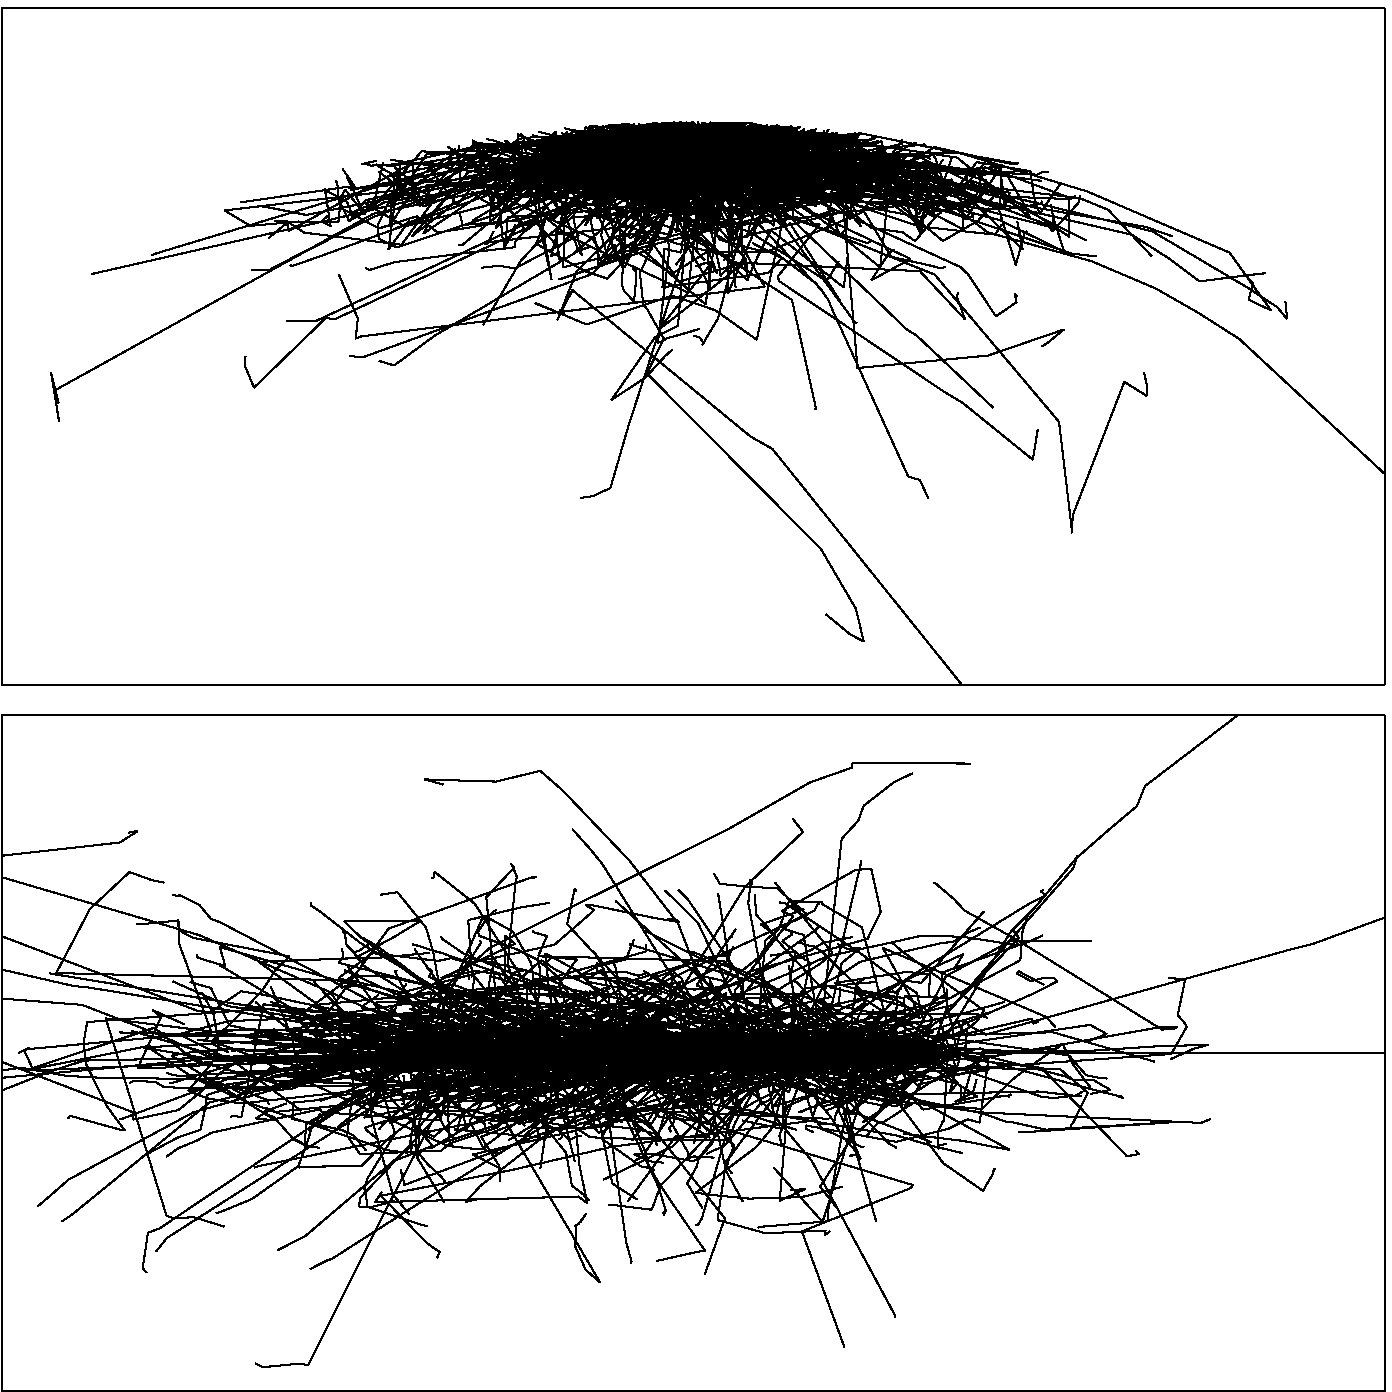
\includegraphics[width=0.6\textwidth]{images/sirotraje.pdf}
    \caption{Siro simulation of the photon paths in the atmosphere in limb-viewing geometry. Upper panel: view from the instrument. Lower panel: view from above. 
      The simulation was run for the 30~km tangent height using 1000 photons.}
    \label{siro_trajectories}
\end{figure}


% references:

\bibliographystyle{plainnat}

\begingroup
\let\cleardoublepage\clearpage
\bibliography{references}
\endgroup

%\iffalse

% include papers
%\setboolean{@twoside}{false}

\newpage
\clearpage
\thispagestyle{empty}
\mbox{}
%\lipsum[1-12]
\newpage
\clearpage
\thispagestyle{empty}
\vspace*{-4.1cm} \begin{tcolorbox}[left skip=13.8cm,colframe=black,width=1.3cm,height=5cm,colback={black},outer arc=0mm,valign=center]    
  \vspace*{-1cm}\hspace*{-0.01cm}\Huge{\textcolor{white}{I}}
\end{tcolorbox}
\vspace*{2cm}
\noindent{}\textcopyright~2008 American Geophysical Union \\
\\
\noindent{}Reprinted, with permission, from \\
\noindent{}\textit{Journal of Geophysical Research: Atmospheres}, 113, D04308, \\
\noindent{}doi:10.1029/2007JD008591
\newpage
\clearpage
\thispagestyle{empty}
\mbox{}
\newpage
\clearpage
%\includepdf[pages={1-3}]{article1.pdf}
\newpage
\clearpage
\thispagestyle{empty}
\vspace*{2cm} \begin{tcolorbox}[left skip=13.8cm,colframe=black,width=1.3cm,height=5cm,colback={black},outer arc=0mm,valign=center]
  \vspace*{-1cm}\hspace*{-0.16cm}\Huge{\textcolor{white}{II}}
\end{tcolorbox}
\vspace*{-4cm}
\noindent{}\textcopyright~Authors 2011. CC Attribution 3.0 License. \\
\\
\noindent{}Reprinted from \\
\noindent{}\textit{Atmospheric Measurement Techniques}, 4,  659\textendash{}667, \\
\noindent{}doi:10.5194/amt-4-659-2011
\newpage
\clearpage
\thispagestyle{empty}
\mbox{}
\newpage
\clearpage
%\includepdf[pages=1-9]{article2.pdf}
%\newpage
%\clearpage
\thispagestyle{empty}
\mbox{}
%\newpage
%\clearpage
\thispagestyle{empty}
\vspace*{10cm} \begin{tcolorbox}[left skip=13.8cm,colframe=black,width=1.3cm,height=5cm,colback={black},outer arc=0mm,valign=center]
  \vspace*{-1cm}\hspace*{-0.33cm}\Huge{\textcolor{white}{III}}
\end{tcolorbox}
\vspace*{-12cm}
\noindent{}\textcopyright~Authors 2015. CC Attribution 3.0 License. \\
\\
\noindent{}Reprinted from \\
\noindent{}\textit{Atmospheric Measurement Techniques}, 8,  3107\textendash{}3115, \\
\noindent{}doi:10.5194/amt-8-3107-2015
\newpage
\clearpage
\thispagestyle{empty}
\mbox{}
%\includepdf[pages=1-9]{article3.pdf}
%\newpage
%\clearpage
\thispagestyle{empty}
\mbox{}
%\newpage
%\clearpage
\thispagestyle{empty}
\newgeometry{bottom=0mm,inner=25mm,outer=20mm}
\vspace*{16.5cm} \begin{tcolorbox}[left skip=13.8cm,colframe=black,width=1.3cm,height=5cm,colback={black},outer arc=0mm,valign=center]
  \vspace*{-1cm}\hspace*{-0.35cm}\Huge{\textcolor{white}{IV}}
\end{tcolorbox}
\vspace*{-18.1cm}
\noindent{}\textcopyright~2016 American Geophysical Union \\
\\
\noindent{}Reprinted, with permission, from \\
\noindent{}\textit{Journal of Geophysical Research: Atmospheres}, 121, \\
\noindent{}doi:10.1002/2015JD024657
\newpage
\clearpage
\thispagestyle{empty}
\mbox{}
\newpage
\clearpage
%\includepdf[pages=1-16]{article4.pdf}


%\fi

\end{document}
